% =====================================================================
%  Datasheet — Etilômetro Veicular SIGHIR DAD01
%  Compilar com pdfLaTeX (local: MiKTeX · Overleaf: Compiler = pdfLaTeX)
%  Estrutura:  main.tex          documento
%              tex/telas.tex     telas do equipamento (TikZ)
%              tex/desenhos.tex  desenhos técnicos e diagramas (TikZ)
%              images/           fotos, capturas do portal/app e logotipo
% =====================================================================
\documentclass[a4paper,10pt]{article}

% ---------- Idioma, codificação e fontes ----------
\usepackage[utf8]{inputenc}
\usepackage[T1]{fontenc}
\usepackage[brazilian]{babel}
\usepackage{roboto}                    % fonte do display do equipamento (telas)
\usepackage[default]{sourcesanspro}    % fonte do documento
\usepackage[scaled=0.86]{zi4}
\usepackage{textcomp}
\usepackage{amssymb}
\usepackage{microtype}
\linespread{1.05}

% ---------- Página ----------
\usepackage[a4paper,top=25mm,bottom=21mm,left=16mm,right=16mm,headheight=14mm,headsep=6mm,footskip=10mm]{geometry}
\usepackage{fancyhdr}
\usepackage{lastpage}

% ---------- Cores, gráficos e caixas ----------
\usepackage[table]{xcolor}
\usepackage{graphicx}
\graphicspath{{images/}}
\usepackage{tikz}
\usetikzlibrary{positioning,calc,arrows.meta,decorations.pathmorphing}
\usepackage[skins,breakable]{tcolorbox}

% ---------- Tabelas, listas, títulos ----------
\usepackage{array}
\usepackage{tabularx}
\usepackage{multicol}
\usepackage{enumitem}
\usepackage{titlesec}
\usepackage[font=footnotesize,labelfont={bf,color=sgreendark},labelsep=endash,skip=4pt]{caption}

\usepackage[hidelinks,pdftitle={Datasheet - Etilômetro Veicular SIGHIR DAD01},pdfauthor={SIGHIR}]{hyperref}

% ---------- Identidade visual ----------
\definecolor{sgreen}{HTML}{68B332}
\definecolor{sgreendark}{HTML}{3F7A1C}
\definecolor{sgreenlight}{HTML}{EEF6E8}
\definecolor{sdark}{HTML}{1F2A24}
\definecolor{sgray}{HTML}{5F6B66}
\definecolor{slight}{HTML}{F4F6F3}
\definecolor{sline}{HTML}{D5DCD2}
\definecolor{salert}{HTML}{C0392B}
\definecolor{samber}{HTML}{D68910}

% =====================================================================
%  Telas do etilômetro DAD01 desenhadas em vetor (TikZ)
%  Baseadas no firmware v6.4.8: tela 320 x 480 px (retrato), textos de
%  device/lang (PT), posições e cores de objects/display e objects/test.
%  Coordenadas em pixels da tela, y para baixo. Para legibilidade no papel
%  as fontes foram ampliadas e textos longos quebrados em mais linhas.
% =====================================================================

% Cores do display (RGB565 do firmware convertido para RGB)
\definecolor{tftgreen}{RGB}{22,178,52}    % TFT_GREEN (tom do LCD)
\definecolor{tftred}{RGB}{214,24,24}      % TFT_RED
\definecolor{tftorange}{RGB}{240,160,0}   % TFT_ORANGE
\definecolor{tftyellow}{RGB}{33,157,90}   % YELLOW  (0x24EB)
\definecolor{tftdgrey}{RGB}{38,37,38}     % DARK_GREY (0x2104)
% Moldura (cor da carcaça)
\definecolor{dadbody}{HTML}{3AA64C}
\definecolor{dadbodyedge}{HTML}{1A9530}
\definecolor{dadlogo}{HTML}{318E41}

% Fontes Roboto (as mesmas do display)
\newcommand{\fA}{\fontsize{12}{13}\roboto\selectfont}                      % títulos
\newcommand{\fB}{\fontsize{11.5}{12.5}\roboto\bfseries\selectfont}         % botões
\newcommand{\fC}{\fontsize{10}{11}\roboto\robotocondensed}                 % textos auxiliares

\tikzset{dadpx/.style={x=0.125mm,y=-0.125mm,every node/.style={inner sep=0pt,outer sep=0pt,anchor=center,align=center}}}

% \dad[largura]{conteúdo da tela}
\newcommand{\dad}[2][27mm]{%
  \resizebox{#1}{!}{%
  \begin{tikzpicture}[dadpx]
    % bocal lateral
    \draw[fill=dadbody,draw=black!75,line width=0.5pt,rounded corners=0.8mm] (-62,44) rectangle (-40,114);
    % corpo
    \draw[fill=dadbody,draw=black!75,line width=0.6pt,rounded corners=4mm] (-40,-50) rectangle (360,690);
    % moldura da tela
    \draw[fill=black!85,draw=black!75,line width=0.4pt,rounded corners=1.2mm] (-12,-14) rectangle (332,494);
    \begin{scope}
      \clip (0,0) rectangle (320,480);
      \fill[black] (0,0) rectangle (320,480);
      #2
    \end{scope}
    % logotipo em baixo relevo
    \node[text=dadlogo,font=\fontsize{30}{30}\roboto\bfseries\itshape\selectfont] at (160,592) {SIGHIR};
  \end{tikzpicture}}}

% Barra de progresso (LoadingWindow::drawBar): y = topo, #2 = fração 0..1
\newcommand{\dadbarra}[2]{%
  \fill[white] (32,#1) rectangle (288,{#1+26});
  \fill[black] (35,{#1+3}) rectangle (285,{#1+23});
  \fill[white] (35,{#1+3}) rectangle ({35+250*#2},{#1+23});}

% Aviso legal exibido durante câmera e análise (TestScreens::inmetro)
\newcommand{\dadinmetro}{%
  \node[white,font=\fC] at (160,178) {Este dispositivo não se};
  \node[white,font=\fC] at (160,212) {enquadra no âmbito};
  \node[white,font=\fC] at (160,246) {probatório de fiscalização};
  \node[white,font=\fC] at (160,280) {ou qualquer outro tipo};
  \node[white,font=\fC] at (160,314) {de punição legal};
  \node[white,font=\fC] at (160,410) {Portaria INMETRO Nº369};}

% ---------------- Telas ----------------
\newcommand{\telaIniciado}{%
  \node[white,font=\fA] at (160,225) {Teste Iniciado};
  \node[white,font=\fC] at (160,322) {clique na tela para};
  \node[tftred,font=\fC] at (160,352) {Adiamento de Emergência};
  \node[white,font=\fC] at (160,433) {iniciando em: 3};}

\newcommand{\telaCamera}{%
  \node[white,font=\fA] at (160,44) {Aguardando Câmera};
  \dadbarra{76}{0.4}
  \node[white,font=\fC] at (160,128) {40\%};
  \dadinmetro}

\newcommand{\telaCalibrando}{%
  \node[tftred,font=\fC] at (160,46) {21480 - 27 ºC};
  \node[white,font=\fA] at (160,190) {Calibrando};
  \node[white,font=\fA] at (160,226) {Sensor};
  \dadbarra{264}{0.68}
  \node[white,font=\fC] at (160,316) {68\%};
  \node[white,font=\fC] at (160,380) {Toque Para Adiar};}

\newcommand{\telaAssopre}{%
  \node[white,font=\fontsize{15}{16}\roboto\selectfont] at (160,225) {Assopre};}

\newcommand{\telaAnalisando}{%
  \node[white,font=\fA] at (160,40) {Analisando};
  \dadbarra{70}{0.55}
  \node[white,font=\fC] at (160,122) {55\%};
  \dadinmetro}

\newcommand{\telaResultado}{%
  \node[white,font=\fontsize{14}{15}\roboto\selectfont] at (160,225) {0.000 mg/L};
  \node[tftred,font=\fA] at (160,423) {21875};}

\newcommand{\telaLiberado}{%
  \fill[tftgreen] (0,0) rectangle (320,480);
  \node[white,font=\fB] at (160,205) {Veículo};
  \node[white,font=\fB] at (160,245) {Desbloqueado};}

\newcommand{\telaAlcool}{%
  \fill[tftred] (0,0) rectangle (320,480);
  \node[white,font=\fB] at (160,205) {Álcool};
  \node[white,font=\fB] at (160,245) {Detectado};}

\newcommand{\telaOpcoes}{%
  \fill[tftyellow] (0,0) rectangle (320,160);
  \fill[tftdgrey] (0,160) rectangle (320,320);
  \fill[white] (0,320) rectangle (320,480);
  \node[white,font=\fB] at (160,80) {Contrassenha};
  \node[tftyellow!70!white,font=\fB] at (160,222) {Realizar};
  \node[tftyellow!70!white,font=\fB] at (160,258) {Outro Teste};
  \node[black,font=\fB] at (160,382) {Desligar};
  \node[black,font=\fB] at (160,418) {Display};}

\newcommand{\dadtecla}[3]{% x, y, rótulo
  \fill[white] (#1,#2) rectangle ({#1+50},{#2+50});
  \node[black,font=\fB] at ({#1+25},{#2+25}) {#3};}

\newcommand{\telaSenha}{%
  \node[white,font=\fB] at (165,40) {Contrassenha};
  \fill[white] (40,60) rectangle (290,105);
  \node[black,font=\fB] at (165,83) {4721};
  \node[white,font=\fB] at (165,130) {Digite};
  \fill[white] (40,150) rectangle (290,195);
  \dadtecla{80}{220}{1}\dadtecla{140}{220}{2}\dadtecla{200}{220}{3}
  \dadtecla{80}{280}{4}\dadtecla{140}{280}{5}\dadtecla{200}{280}{6}
  \dadtecla{80}{340}{7}\dadtecla{140}{340}{8}\dadtecla{200}{340}{9}
  \dadtecla{80}{400}{<}\dadtecla{140}{400}{0}\dadtecla{200}{400}{+}
  \dadtecla{260}{340}{\^{}}\dadtecla{260}{400}{OK}}

\newcommand{\telaRandomico}{%
  \fill[tftyellow] (0,0) rectangle (320,240);
  \fill[tftdgrey] (0,240) rectangle (320,480);
  \node[white,font=\fB] at (160,120) {Iniciar Teste};
  \node[tftyellow!70!white,font=\fB] at (160,360) {Adiar};}

\newcommand{\telaMotorista}{%
  \fill[tftred] (0,0) rectangle (320,480);
  \node[white,font=\fB] at (160,190) {MOTORISTA};
  \node[white,font=\fB] at (160,226) {NÃO};
  \node[white,font=\fB] at (160,262) {AUTORIZADO};
  \node[white,font=\fC] at (160,360) {Estacione o veículo};}

% Tela com legenda numerada embaixo: \dadfig[largura]{tela}{nº}{legenda}
\newcommand{\dadfig}[4][27mm]{%
  \begin{minipage}[t]{#1}\centering
    \dad[#1]{#2}\\[1.5mm]
    {\footnotesize\textbf{\color{sgreendark}#3}\enspace\color{sdark}#4}
  \end{minipage}}

% =====================================================================
%  Desenhos técnicos do DAD01 em vetor (TikZ) — estilo de desenho técnico
%  Medidas em mm.
% =====================================================================

\definecolor{fiomarrom}{HTML}{7B4A26}
\definecolor{fiolaranja}{HTML}{F08A1C}
\definecolor{fioverde}{HTML}{2E9E3E}
\definecolor{fiovermelho}{HTML}{D42A2A}
\definecolor{tdline}{HTML}{262626}
\definecolor{tdfill}{HTML}{F2F2F2}
\definecolor{tddim}{HTML}{4D4D4D}

\tikzset{
  td/.style={draw=tdline,line width=0.55pt},
  tdfino/.style={draw=tdline,line width=0.3pt},
  tdoculto/.style={draw=tdline!70,line width=0.3pt,dash pattern=on 1.2pt off 0.8pt},
  tdeixo/.style={draw=tdline!60,line width=0.25pt,dash pattern=on 4pt off 1pt on 0.6pt off 1pt},
  cota/.style={tddim,line width=0.3pt,{Stealth[length=1.5mm,width=0.8mm]}-{Stealth[length=1.5mm,width=0.8mm]}},
  aux/.style={tddim,line width=0.25pt},
  rot/.style={font=\scriptsize,text=tdline,fill=white,inner sep=0.8pt},
  vista/.style={font=\tiny\bfseries,text=tddim},
  chamada/.style={circle,draw=tdline,line width=0.4pt,fill=white,font=\tiny\bfseries,inner sep=0pt,minimum size=3.6mm},
  lider/.style={tdline,line width=0.3pt},
}

% ---------------- Unidade exposta: vistas frontal e lateral ----------------
\newcommand{\desenhoExposta}{%
\begin{tikzpicture}[x=0.36mm,y=0.36mm]
  % vista frontal
  \draw[td,fill=white,rounded corners=0.6mm] (-8.5,84.4) rectangle (0,94.9);           % bocal
  \draw[td,fill=white,rounded corners=2mm] (0,0) rectangle (62.3,112.5);
  \draw[tdfino,rounded corners=0.8mm] (6.7,31.1) rectangle (55.6,104.5);              % moldura da tela
  \draw[tdfino,fill=tdfill] (9,34) rectangle (53.3,101.6);                            % área ativa
  \node[font=\tiny\itshape\bfseries,text=tdline!60] at (31.15,15) {SIGHIR};
  % vista lateral
  \draw[td,fill=white,rounded corners=1.6mm] (80,0) rectangle (109,112.5);
  \draw[tdfino] (84,4) -- (84,108.5);
  \draw[tdoculto] (80,84.4) -- (109,84.4); \draw[tdoculto] (80,94.9) -- (109,94.9);
  % cotas
  \draw[aux] (0,114) -- (0,123); \draw[aux] (62.3,114) -- (62.3,123);
  \draw[cota] (0,120) -- node[rot]{62,3} (62.3,120);
  \draw[aux] (80,114) -- (80,123); \draw[aux] (109,114) -- (109,123);
  \draw[cota] (80,120) -- node[rot]{29,0} (109,120);
  \draw[aux] (110.5,0) -- (120,0); \draw[aux] (110.5,112.5) -- (120,112.5);
  \draw[cota] (117,0) -- node[rot,rotate=90]{112,5} (117,112.5);
  \node[vista] at (31.15,-9) {VISTA FRONTAL};
  \node[vista] at (94.5,-9) {VISTA LATERAL};
\end{tikzpicture}}

% ---------------- Unidade embutida: vistas superior e lateral ----------------
\newcommand{\dbnove}[3]{% x, y (base), largura — conector DB9 em vista superior
  \draw[tdfino,fill=white] (#1,#2) rectangle ({#1+#3},{#2+2.2});
  \draw[tdfino,fill=tdfill] ({#1+2.2},{#2+2.2}) -- ({#1+#3-2.2},{#2+2.2}) -- ({#1+#3-3.4},{#2+6.5}) -- ({#1+3.4},{#2+6.5}) -- cycle;}
\newcommand{\desenhoEmbutida}{%
\begin{tikzpicture}[x=0.33mm,y=0.33mm]
  % vista superior
  \draw[td,fill=white,rounded corners=1mm] (122,24) -- (129,27) -- (129,61) -- (122,64);  % orelha
  \draw[tdfino,rounded corners=0.8mm] (123.5,34) rectangle (126.5,54);
  \draw[td,fill=white,rounded corners=3mm] (0,0) rectangle (122,88);
  \draw[tdfino,rounded corners=2mm] (14,10) rectangle (108,72);
  \dbnove{12}{88}{22}
  \draw[tdfino,fill=white] (44,88) rectangle (56,93);                                   % Microfit 8
  \draw[tdfino,fill=white] (76,88) rectangle (85,93);                                   % Microfit 6
  % vista lateral
  \draw[td,fill=white,rounded corners=1.5mm] (0,-46) rectangle (122,-18);
  \draw[tdfino] (0,-26) -- (122,-26);
  % cotas
  \draw[aux] (0,96) -- (0,106); \draw[aux] (129,63) -- (129,106);
  \draw[cota] (0,103) -- node[rot]{129} (129,103);
  \draw[aux] (-1.5,0) -- (-11,0); \draw[aux] (-1.5,88) -- (-11,88);
  \draw[cota] (-8,0) -- node[rot,rotate=90]{88} (-8,88);
  \draw[aux] (-1.5,-46) -- (-11,-46); \draw[aux] (-1.5,-18) -- (-11,-18);
  \draw[cota] (-8,-46) -- node[rot,rotate=90]{28} (-8,-18);
  \node[vista] at (61,40) {VISTA SUPERIOR};
  \node[vista] at (61,-53) {VISTA LATERAL};
\end{tikzpicture}}

% ---------------- Conector Microfit 6 vias (vista frontal, lado do cabo) ----------------
\newcommand{\desenhoConector}{%
\begin{tikzpicture}[x=1mm,y=1mm]
  \draw[td,fill=white,rounded corners=0.5mm] (-1.5,-1.5) rectangle (22.5,14.5);
  \draw[td,fill=white] (7,14.5) rectangle (14,17.5);                                    % trava
  \foreach \i/\x/\y in {1/0/0, 2/7.5/0, 3/15/0, 4/0/7.5, 5/7.5/7.5, 6/15/7.5} {
    \draw[tdfino,fill=tdfill] (\x,\y) rectangle ({\x+6},{\y+6});
    \node[font=\scriptsize\bfseries,text=tdline] at ({\x+3},{\y+3}) {\i};}
  \node[vista] at (10.5,-4.3) {VISTA DO ENCAIXE};
\end{tikzpicture}}

% ---------------- Diagrama de ligação no veículo ----------------
\newcommand{\figuraIntegracao}{%
\begin{tikzpicture}[x=1mm,y=1mm,
  bloco/.style={td,fill=white,align=center,font=\scriptsize},
  titb/.style={font=\scriptsize\bfseries,text=tdline,align=center},
  porta/.style={font=\tiny,text=tddim},
  fio/.style={tdline,line width=0.55pt},
  ser/.style={tdline,line width=1.1pt}]
  % --- chave de ignição e relé de bloqueio
  \draw[td,fill=white] (0,30) rectangle (26,40);
  \node[titb] at (13,35) {CHAVE DE IGNIÇÃO\\[-1pt]{\normalfont\tiny pós-chave}};
  \draw[fio] (13,30) -- (13,27.5);
  \fill[tdline] (13,27.5) circle (0.45); \node[porta,anchor=east] at (12.4,27.5) {30};
  \draw[fio] (13,27.5) -- (14.6,23.6);                                                   % contato NF
  \fill[tdline] (13,23.5) circle (0.45); \node[porta,anchor=east] at (12.4,23.5) {87a};
  \draw[fio] (13,23.5) -- (13,20);
  \draw[td,fill=white] (0,10) rectangle (26,20);
  \node[titb] at (13,15) {CIRCUITO DE\\[-1pt]PARTIDA};
  % bobina do relé
  \draw[td,fill=white] (20,23) rectangle (28,28); \draw[tdfino] (20,23) -- (28,28);
  \node[porta,anchor=north] at (24,22.6) {K1 (85/86)};
  \draw[tdoculto] (15,25.5) -- (20,25.5);
  % --- rastreador
  \draw[td,fill=white] (46,8) rectangle (80,42);
  \node[titb] at (63,38) {RASTREADOR};
  \node[font=\tiny,text=tddim] at (63,34.5) {MiX · Suntech · Entrack};
  \draw[fio] (26,36.5) -- (46,36.5); \node[porta,anchor=south west] at (46.6,36.6) {IGN};
  \fill[tdline] (26,36.5) circle (0.45);
  \draw[fio] (28,25.5) -- (46,25.5); \node[porta,anchor=south west] at (46.6,25.6) {SAÍDA BLOQ.};
  \draw[ser] (80,25) -- (100,25); \node[porta,anchor=south] at (90,25.4) {RS232 · 115.200 bps};
  % --- unidade embutida
  \draw[td,fill=white] (100,8) rectangle (134,42);
  \node[titb] at (117,38) {UNIDADE\\[-1pt]EMBUTIDA};
  \node[porta,anchor=west] at (100.8,25) {DB9 M};
  \node[porta,anchor=east] at (133.2,25) {MICROFIT 8};
  \node[porta,anchor=south] at (117,8.6) {MICROFIT 6};
  \draw[ser] (134,25) -- (152,25); \node[porta,anchor=south] at (143,25.4) {espiral 8 vias};
  % --- unidade exposta
  \draw[td,fill=white] (152,8) rectangle (178,42);
  \node[titb] at (165,25) {UNIDADE\\[-1pt]EXPOSTA};
  % --- alimentação
  \draw[td,fill=white] (0,-6) rectangle (26,4);
  \node[titb] at (13,-1) {BATERIA\\[-1pt]{\normalfont\tiny 12/24 V}};
  \draw[fio] (26,-1) -- (64,-1);
  \draw[td,fill=white] (64,-2.5) rectangle (72,0.5); \node[porta,anchor=north] at (68,-3) {F 7,5 A};
  \draw[fio] (72,-1) -- (117,-1) -- (117,8);
  \node[porta,anchor=south west] at (118,1) {VCC / GND};
\end{tikzpicture}}

% ---------------- Unidade embutida: vista interna com componentes ----------------
\newcommand{\desenhoEmbutidaInterna}{%
\begin{tikzpicture}[x=0.51mm,y=0.51mm]
  % caixa e orelha
  \draw[td,fill=white,rounded corners=1mm] (122,22) -- (131,26) -- (131,58) -- (122,62);
  \draw[tdfino,rounded corners=0.8mm] (125,32) rectangle (128,52);
  \draw[td,fill=white,rounded corners=3mm] (0,0) rectangle (122,88);
  % placa
  \draw[tdfino,fill=tdfill,rounded corners=1mm] (5,5) rectangle (117,80);
  \foreach \p in {(9,9),(113,9),(9,76),(113,76)} \draw[tdfino,fill=white] \p circle (1.6);
  % DB9 macho (vista superior, flange + corpo em D)
  \draw[tdfino,fill=white] (10,80) rectangle (44,83.5);
  \draw[tdfino,fill=white] (15,83.5) -- (39,83.5) -- (37,94) -- (17,94) -- cycle;
  \foreach \x in {19,23,27,31,35} \fill[tdline] (\x,91) circle (0.75);
  \foreach \x in {21,25,29,33} \fill[tdline] (\x,87) circle (0.75);
  \draw[tdfino,fill=white] (12,81.75) circle (1.3); \draw[tdfino,fill=white] (42,81.75) circle (1.3);
  % Microfit 8 e 6
  \draw[tdfino,fill=white] (52,72) rectangle (70,88);
  \foreach \x in {54.5,58.5,62.5,66.5} {\draw[tdfino] (\x,75) rectangle ({\x+3},78.5); \draw[tdfino] (\x,81) rectangle ({\x+3},84.5);}
  \draw[tdfino,fill=white] (78,72) rectangle (92,88);
  \foreach \x in {80.5,84.5,88} {\draw[tdfino] (\x,75) rectangle ({\x+2.6},78.5); \draw[tdfino] (\x,81) rectangle ({\x+2.6},84.5);}
  % CI interface RS232 (SOIC)
  \draw[tdfino,fill=white] (18,46) rectangle (34,58); \draw[tdfino] (19.5,56.5) circle (0.6);
  \foreach \y in {47.5,50,52.5,55} {\draw[tdfino] (16.5,\y) -- (18,\y); \draw[tdfino] (34,\y) -- (35.5,\y);}
  % relé
  \draw[tdfino,fill=white] (50,14) rectangle (74,34);
  \node[font=\tiny,text=tddim] at (62,24) {K1};
  % capacitor eletrolítico
  \draw[tdfino,fill=white] (60,56) circle (6); \draw[tdfino] (60,56) circle (4.6);
  % reguladores: indutor + trimpot
  \foreach \y in {14,34,54} {
    \draw[tdfino,fill=white] (96,\y) rectangle (108,{\y+12});
    \draw[tdfino] (102,{\y+6}) circle (3.2);
    \draw[tdfino] (100.4,{\y+6}) -- (103.6,{\y+6});}
  % chamadas
  \draw[lider] (27,94) -- (27,101) node[chamada,above] {1};
  \draw[lider] (61,88) -- (61,101) node[chamada,above] {2};
  \draw[lider] (85,88) -- (85,101) node[chamada,above] {3};
  \draw[lider] (18,52) -- (-6,52) node[chamada,left] {4};
  \draw[lider] (50,24) -- (-6,24) node[chamada,left] {5};
  \draw[lider] (102,66) -- (102,101) node[chamada,above] {6};
  \draw[lider] (129,30) -- (129,-7) node[chamada,below] {7};
\end{tikzpicture}}


\newcommand{\docrev}{Rev.~5.1}
\newcommand{\docdate}{Outubro de 2026}
\newcommand{\fw}{v6.4.8}

\setlength{\parindent}{0pt}
\setlength{\parskip}{5pt}
\renewcommand{\arraystretch}{1.25}
\setlength{\columnsep}{8mm}
\setlength{\tabcolsep}{4.5pt}
\color{sdark}

% ---------- Cabeçalho e rodapé ----------
\pagestyle{fancy}
\fancyhf{}
\fancyhead[L]{\raisebox{-1.2mm}{
\includegraphics[height=6.5mm]{logo.png}}}
\fancyhead[R]{\footnotesize\color{sgray}\textbf{\color{sdark}Etilômetro Veicular DAD01}\enspace|\enspace Datasheet \docrev}
\renewcommand{\headrule}{{\color{sgreen}\hrule height 0.9pt}\vspace{-0.9pt}}
\fancyfoot[L]{\scriptsize\color{sgray}SIGHIR \,·\, sighir.com \,·\, contato@sighir.com.br}
\fancyfoot[C]{\scriptsize\color{sgray}\docdate}
\fancyfoot[R]{\scriptsize\color{sgray}Página \thepage\ de \pageref{LastPage}}
\renewcommand{\footrulewidth}{0.4pt}
\renewcommand{\footrule}{{\color{sline}\hrule height 0.4pt}\vspace{2pt}}

% ---------- Títulos ----------
\titleformat{\section}
  {\normalfont\large\bfseries\color{sdark}}
  {\colorbox{sgreen}{\makebox[5.5mm][c]{\color{white}\thesection}}}
  {2.5mm}{\MakeUppercase}
  [\vspace{-1.2mm}{\color{sgreen}\rule{\linewidth}{0.8pt}}]
\titlespacing*{\section}{0pt}{12pt}{6pt}
\titleformat{\subsection}
  {\normalfont\normalsize\bfseries\color{sgreendark}}{\thesubsection}{2mm}{}
\titlespacing*{\subsection}{0pt}{9pt}{3pt}

% ---------- Listas ----------
\setlist{nosep,leftmargin=4.5mm,itemsep=2pt}
\setlist[itemize]{label={\color{sgreen}\scriptsize$\blacktriangleright$}}
\setlist[enumerate]{label={\color{sgreendark}\bfseries\arabic*.},leftmargin=5.5mm}

% ---------- Caixas ----------
\newtcolorbox{nota}[1][]{enhanced,breakable,colback=sgreenlight,colframe=sgreen,boxrule=0pt,
  leftrule=2.5pt,arc=0pt,outer arc=0pt,left=7pt,right=7pt,top=5pt,bottom=5pt,fontupper=\small,
  before skip=7pt,after skip=7pt,#1}
\newtcolorbox{alerta}[1][]{enhanced,breakable,colback=slight,colframe=samber,boxrule=0pt,
  leftrule=2.5pt,arc=0pt,outer arc=0pt,left=7pt,right=7pt,top=5pt,bottom=5pt,fontupper=\small,
  before skip=7pt,after skip=7pt,#1}

% ---------- Atalhos ----------
\newcommand{\ev}[1]{\texttt{\$ETEV#1!}}
\newcommand{\tela}[1]{\textbf{«#1»}}
\newcommand{\hl}[1]{\textbf{\color{sgreendark}#1}}
\newcommand{\seta}{\,$\rightarrow$\,}
\newcommand{\opc}{\tcbox[on line,colback=sline!60,colframe=sline!60,arc=0.8mm,boxsep=0pt,left=2pt,right=2pt,top=1pt,bottom=1pt,fontupper=\tiny\bfseries\color{sgray}]{OPCIONAL}}
\newcolumntype{L}{>{\raggedright\arraybackslash}X}
\newcolumntype{P}[1]{>{\leavevmode\raggedright\arraybackslash}p{#1}}
\newcolumntype{G}[1]{>{\leavevmode\color{sgray}\raggedright\arraybackslash}p{#1}}
\newcolumntype{B}[1]{>{\leavevmode\bfseries\raggedright\arraybackslash}p{#1}}
\newcommand{\thead}[1]{\textbf{\color{white}#1}}
\newcommand{\headrow}{\rowcolor{sdark}}
\newcommand{\grupo}[1]{\rowcolor{sgreenlight}\multicolumn{2}{@{\hspace{2pt}}l}{\textbf{\color{sgreendark}\scriptsize\MakeUppercase{#1}}}\\}

% Passo numerado da faixa "como funciona"
\newcommand{\passo}[3]{%
  \begin{tcolorbox}[enhanced,width=\linewidth,colback=white,colframe=sline,boxrule=0.6pt,arc=1.5mm,
    left=5pt,right=5pt,top=4pt,bottom=4pt,height=21mm,valign=top,
    borderline north={2.5pt}{0pt}{sgreen}]
    {\Large\bfseries\color{sgreen}#1}\enspace{\small\bfseries #2}\par\vspace{2pt}
    {\scriptsize\color{sgray}#3}
  \end{tcolorbox}}

% Indicador da faixa escura da capa
\newcommand{\kpi}[2]{\makebox[\linewidth][c]{\large\bfseries\color{sgreen}#1}\par\vspace{2pt}\makebox[\linewidth][c]{\footnotesize\color{white!85!sdark}#2}}

\begin{document}

% =====================================================================
%  PÁGINA 1 — APRESENTAÇÃO
% =====================================================================
{\footnotesize\bfseries\color{sgreendark}DATASHEET \,·\, \docrev \,·\, FIRMWARE \fw}\\[3mm]
{\fontsize{28}{33}\selectfont\bfseries Etilômetro Veicular SIGHIR DAD01}\\[3.5mm]
\begin{minipage}{0.85\textwidth}
{\large\color{sgray}Bafômetro de ignição com sensor calibrado e verificação redundante por IA, bloqueio
de partida, testes randômicos e rastreabilidade completa de eventos.}
\end{minipage}

\vspace{5mm}
\begin{tcolorbox}[enhanced,colback=sdark,colframe=sdark,arc=1.5mm,left=2mm,right=2mm,top=3mm,bottom=3mm,fontupper=\color{white}]
\renewcommand{\arraystretch}{1}
\begin{tabularx}{\linewidth}{@{}*{5}{>{\centering\arraybackslash}X}@{}}
\kpi{Antipartida}{nunca desliga em viagem} &
\kpi{Dupla verificação}{sensor calibrado + IA} &
\kpi{0,03\,mg/L}{precisão de medição} &
\kpi{1 ano · 2.500}{validade (sopros)} &
\kpi{RS232 + Wi-Fi}{comunicação}\\
\end{tabularx}
\end{tcolorbox}

\begin{multicols}{2}
\section{Visão geral}

O \textbf{SIGHIR DAD01} é um etilômetro veicular embarcado (bafômetro de ignição) que
\hl{condiciona a partida do veículo a um teste de alcoolemia negativo}. A cada partida o
motorista realiza um teste de sopro no próprio equipamento: com resultado negativo o veículo é
liberado; com álcool detectado, permanece bloqueado. Durante a viagem o equipamento solicita
\hl{testes randômicos}, que confirmam que quem conduz é quem foi testado.

Integrado ao rastreador (telemetria) do veículo, o DAD01 transmite cada teste, resultado,
bloqueio e alerta para a plataforma SIGHIR, onde o gestor acompanha a frota, recebe alertas,
emite relatórios e comprova a calibração de cada sensor.

\subsection*{Destaques}
\begin{itemize}
  \item \textbf{Sensor calibrado com redundância por IA}: a medição é confirmada por inteligência artificial embarcada antes de qualquer resultado positivo.
  \item Sensor substituível com \textbf{calibração individual} rastreável e certificado digital.
  \item Bloqueio no circuito de ignição, integrado às telemetrias MiX Telematics, Suntech e Entrack.
  \item Testes randômicos, adiamento limitado e tempo de manobra configuráveis.
  \item Mais de 30 tipos de eventos rastreáveis por equipamento, sensor e veículo.
  \item Firmware e parâmetros atualizáveis remotamente, sob controle da SIGHIR.
\end{itemize}

\columnbreak
\section{Aplicação no transporte de cargas}

No transporte rodoviário de cargas o motorista conduz veículos pesados, em longas jornadas e
longe da supervisão direta. O DAD01 leva para a cabine uma \textbf{barreira técnica e
auditável} contra a condução sob efeito de álcool:

\begin{itemize}
  \item \textbf{Na partida:} o caminhão só funciona após um teste negativo.
  \item \textbf{Na estrada:} testes randômicos impedem que outra pessoa sopre no lugar do condutor.
  \item \textbf{Na gestão:} cada ocorrência chega ao portal com placa, horário e posição — e com vídeo, quando há câmera integrada.
  \item \textbf{Na auditoria:} histórico de testes e certificados de calibração prontos para fiscalizações, embarcadores e seguradoras.
\end{itemize}

\subsection*{Benefícios para a transportadora}
\begin{itemize}
  \item Prevenção de acidentes graves e proteção do motorista e de terceiros.
  \item Menor exposição a responsabilidade civil, sinistros e perdas de carga.
  \item Evidência objetiva para programas de segurança, gerenciamento de risco e exigências de clientes.
  \item Mudança de cultura: o motorista sabe que todo teste é registrado.
  \item Gestão centralizada da frota, sem depender de verificações manuais.
\end{itemize}
\end{multicols}

\vfill
{\small\bfseries\color{sgreendark}COMO FUNCIONA}\par\vspace{1.5mm}
\begin{minipage}[t]{0.235\textwidth}\passo{1}{Ignição}{Ao ligar a chave com o veículo bloqueado, o equipamento solicita o teste.}\end{minipage}\hfill
\begin{minipage}[t]{0.235\textwidth}\passo{2}{Sopro}{Sopro contínuo de 3\,s, validado por sensor de pressão e IA.}\end{minipage}\hfill
\begin{minipage}[t]{0.235\textwidth}\passo{3}{Análise}{O sensor calibrado mede o mg/L e a IA confirma se é álcool.}\end{minipage}\hfill
\begin{minipage}[t]{0.235\textwidth}\passo{4}{Decisão}{Libera ou mantém bloqueado e envia o evento à plataforma.}\end{minipage}

% =====================================================================
%  PÁGINA 2 — ESPECIFICAÇÕES
% =====================================================================
\newpage
\section{Especificações técnicas}

\begin{minipage}[t]{0.49\textwidth}
\small
\begin{tabularx}{\linewidth}[t]{@{}G{27mm}L@{}}
\grupo{Equipamento}
Modelo & DAD01 — etilômetro veicular com bloqueio de partida\\
Composição & Unidade exposta (interface), unidade embutida (alimentação e comunicação) e cabo espiral de 8 vias\\
Processamento & Microcontrolador dual-core 240\,MHz\\
Firmware & \fw{}, atualizável remotamente\\
\grupo{Medição de álcool}
Sensor & Semicondutor aquecido, em módulo substituível com memória própria (ID único, calibração e contador de sopros)\\
Faixa de medição & 0,000 a 2,500\,mg/L de ar expirado\\
Precisão & 0,03\,mg/L\\
Resolução & 0,001\,mg/L\\
Bloqueio & \textbf{De partida}: impede ligar o veículo; nunca desliga o motor em movimento (seção~\ref{sec:bloqueio})\\
Redundância & IA embarcada (\emph{random forest} de 544 árvores) confirma que a leitura é de álcool\\
Tempo de sopro & 3\,s, com no mínimo 1,8\,s contínuos\\
Tempo de análise & \textasciitilde23\,s após o sopro\\
Validade do sensor & \textbf{1 ano ou 2.500 sopros}, o que ocorrer primeiro\\
Calibração & Individual, em laboratório SIGHIR, com padrões certificados; certificado digital por sensor\\
Detecção de sopro & Sensor de pressão dedicado + IA embarcada (55 árvores)\\
\end{tabularx}
\end{minipage}\hfill
\begin{minipage}[t]{0.47\textwidth}
\small
\begin{tabularx}{\linewidth}[t]{@{}G{26mm}L@{}}
\grupo{Elétrica}
Alimentação & 10,5 a 40\,V CC (veículos de 12\,V e 24\,V)\\
Corrente máxima & 4,5\,A\\
Proteção & Fusível dedicado no positivo (recomendado 7,5\,A)\\
Conexões & DB9 macho (RS232) · Microfit 8 vias (exposta) · Microfit 6 vias (alimentação)\\
\grupo{Comunicação}
Serial & RS232 (DB9 macho), 115.200\,bps, 8N1 — integração com a telemetria\\
Wi-Fi & IEEE 802.11 b/g/n, 2,4\,GHz (2.412–2.484\,MHz) — instalação, configuração e atualização\\
Serviço & USB, exclusivo da assistência técnica\\
Bluetooth & \textbf{Não possui}\\
Telemetrias & MiX Telematics (MiX 1.0 e MiX 2.0), Suntech e Entrack\\
\grupo{Interface}
Tela & Colorida, sensível ao toque, 3,5 polegadas (320\,×\,480)\\
Sinalização & Sonora multitom e por cores\\
Idiomas & Português, inglês e espanhol\\
\grupo{Ambiente e mecânica}
Temperatura & 0 a 50\,\textdegree C; alerta a 52\,\textdegree C e alerta crítico a 60\,\textdegree C\\
Umidade & Monitorada; alerta acima de 95\,\%\\
Unidade exposta & 112,5\,×\,62,3\,×\,29,0\,mm \,·\, 140\,g\\
Unidade embutida & 129,0\,×\,88,0\,×\,28,0\,mm \,·\, 130\,g\\
\end{tabularx}
\end{minipage}

\begin{nota}
\textbf{Bluetooth:} o DAD01 \textbf{não possui comunicação Bluetooth}. Versões anteriores deste
documento citavam Bluetooth Classic 4.2; o recurso foi descontinuado e não está presente no
firmware atual. A comunicação com sistemas externos é feita exclusivamente por
\textbf{RS232} (operação, via telemetria) e \textbf{Wi-Fi} (instalação, configuração e
atualização) — ver seção~\ref{sec:comunicacao}.
\end{nota}

\subsection*{Conteúdo do kit}
\begin{minipage}[c]{0.44\textwidth}
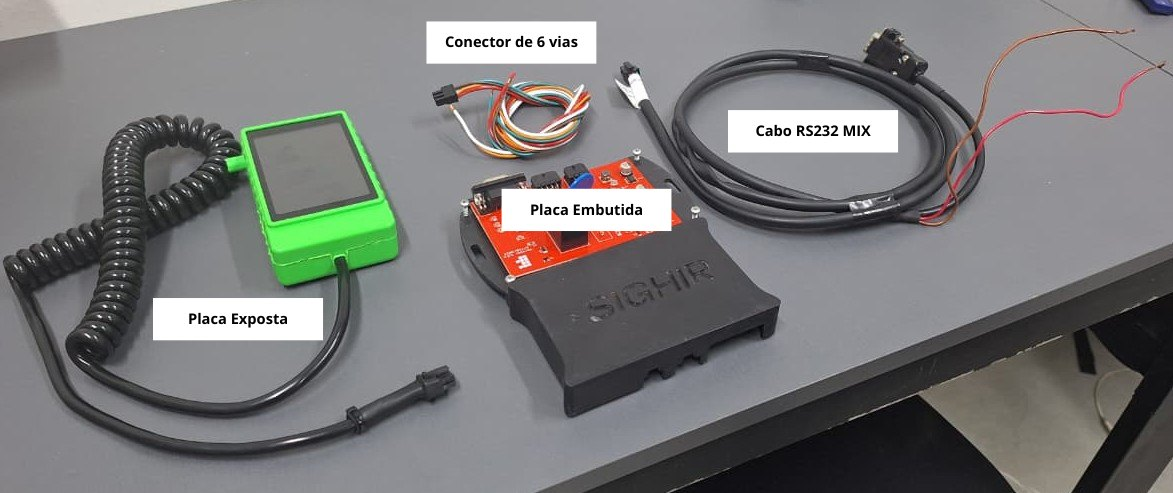
\includegraphics[width=\linewidth]{kit.jpg}
\end{minipage}\hfill
\begin{minipage}[c]{0.52\textwidth}\small
\begin{enumerate}
  \item \textbf{Unidade exposta} — tela, sensor de álcool, sensor de sopro e sensor de temperatura e umidade.
  \item \textbf{Unidade embutida} — regulação de energia, interface RS232 (DB9) e entradas/saídas; instalada oculta atrás do painel.
  \item \textbf{Cabo espiral de 8 vias} — liga a exposta à embutida.
  \item \textbf{Cabo de alimentação de 6 vias} — a partir da bateria ou do módulo de telemetria.
  \item \textbf{Cabo RS232} — específico para a telemetria do veículo.
  \item \textbf{Relé automotivo de bloqueio} com suporte.
\end{enumerate}
\end{minipage}

% =====================================================================
%  PÁGINA 3 — DIMENSÕES E ARQUITETURA
% =====================================================================
\newpage
\section{Dimensões e conexões}
\begin{minipage}[b]{0.31\textwidth}\centering
\desenhoExposta
\captionof{figure}{Unidade exposta (mm).}
\end{minipage}\hfill
\begin{minipage}[b]{0.29\textwidth}\centering
\desenhoEmbutida
\captionof{figure}{Unidade embutida (mm).}
\end{minipage}\hfill
\begin{minipage}[b]{0.34\textwidth}\centering
\desenhoConector\\[3mm]
\footnotesize
\begin{tabularx}{\linewidth}{@{}P{6mm}P{19mm}L@{}}
\headrow \thead{Pino} & \thead{Fio} & \thead{Sinal}\\
1 & {\color{fioverde}\rule{2mm}{2mm}} Verde & Pós-chave \opc\\
\rowcolor{slight} 2 & \fbox{\rule{0mm}{1.3mm}\hspace{1.3mm}} Branco & Entrada auxiliar\\
3 & {\color{fiovermelho}\rule{2mm}{2mm}} Vermelho & VCC (10,5–40\,V)\\
\rowcolor{slight} 4 & {\color{fiomarrom}\rule{2mm}{2mm}} Marrom & GND\\
5 & — & Não conectado\\
\rowcolor{slight} 6 & {\color{fiolaranja}\rule{2mm}{2mm}} Laranja & Relé \opc\\
\end{tabularx}\\[1.5mm]
{\scriptsize\color{sgray}\opc\ com telemetria, o bloqueio é via RS232}
\captionof{figure}{Conector de alimentação (6 vias).}
\end{minipage}

\subsection{Unidade embutida: componentes e conexões}
\begin{minipage}[c]{0.43\textwidth}\centering
\desenhoEmbutidaInterna
\captionof{figure}{Unidade embutida, vista interna (ilustrativa).}
\end{minipage}\hfill
\begin{minipage}[c]{0.54\textwidth}
\footnotesize
\begin{tabularx}{\linewidth}{@{}P{5mm}P{24mm}L@{}}
\headrow \thead{Nº} & \thead{Componente} & \thead{Função}\\
\textbf{1} & \textbf{DB9 macho} & RS232 para a telemetria (115.200\,bps, 8N1), com parafusos de travamento. Recebe cabo com DB9 fêmea: cabo da telemetria ou adaptador USB-RS232 de serviço\\
\rowcolor{slight}\textbf{2} & \textbf{Microfit 8 vias} & Cabo espiral para a unidade exposta: alimentação, serial e sinais\\
\textbf{3} & \textbf{Microfit 6 vias} & Alimentação 10,5–40\,V e entradas/saída opcionais (figura 3)\\
\rowcolor{slight}\textbf{4} & \textbf{Interface RS232} & Conversão de nível da comunicação serial\\
\textbf{5} & \textbf{Relé} & Saída de bloqueio para uso autônomo (opcional)\\
\rowcolor{slight}\textbf{6} & \textbf{Reguladores (3)} & Alimentação da unidade exposta e das entradas; ajustados e verificados em bancada\\
\textbf{7} & \textbf{Orelha de fixação} & Fixação em superfície plana, oculta atrás do painel\\
\end{tabularx}
\end{minipage}

\section{Arquitetura e comunicação}\label{sec:comunicacao}

\begin{center}
\resizebox{\linewidth}{!}{\figuraIntegracao}
\captionof{figure}{Diagrama de ligação do DAD01 no veículo.}
\end{center}

\begin{minipage}[t]{0.47\textwidth}
\setlength{\parskip}{5pt}
Em operação o DAD01 comunica-se com sistemas externos \textbf{por meio do rastreador do
veículo}. A unidade embutida conecta-se à telemetria por \textbf{RS232}: o rastreador informa
ao etilômetro o estado da ignição e executa os comandos de bloqueio e desbloqueio; o etilômetro
envia ao rastreador cada evento codificado (\ev{nn}), que a plataforma da telemetria repassa ao
servidor SIGHIR.

Assim, o equipamento \textbf{não depende de conexão própria à internet} durante a viagem e
aproveita a cobertura já contratada pela frota. O \textbf{Wi-Fi} permanece
\textbf{desabilitado em operação} (padrão de fábrica) e é ativado apenas para instalação,
manutenção e atualização.
\end{minipage}\hfill
\begin{minipage}[t]{0.49\textwidth}
\footnotesize
\begin{tabularx}{\linewidth}[t]{@{}B{14mm}L@{}}
\headrow \thead{Interface} & \thead{Uso}\\
RS232 & Canal operacional com a telemetria: ignição, bloqueio/desbloqueio, eventos e comandos remotos (115.200\,bps)\\
\rowcolor{slight} Wi-Fi & Rede própria do equipamento para o aplicativo SIGHIR Monitor (instalação, parâmetros, troca de sensor, monitoramento local) e conexão à rede da base para atualizações\\
USB & Porta de serviço da assistência técnica (bancada)\\
\end{tabularx}\\[3mm]
\begin{tabularx}{\linewidth}{@{}B{14mm}L@{}}
\headrow \thead{Telemetria} & \thead{Integração}\\
MiX & Ignição e movimento informados por comando serial; bloqueio pelo relé do rastreador\\
\rowcolor{slight} Suntech & Consulta de estado a cada 2\,s; bloqueio por comando ao módulo\\
Entrack & Consulta de ignição a cada 2\,s; bloqueio pela saída do módulo\\
\end{tabularx}
\end{minipage}

% =====================================================================
%  PÁGINA 4 — TECNOLOGIA DE DETECÇÃO (IA + CALIBRAÇÃO)
% =====================================================================
\section{Tecnologia de medição: sensor calibrado e redundância por IA}\label{sec:ia}

A medição do DAD01 é feita pelo \textbf{sensor de álcool com calibração individual}, como em um
etilômetro convencional. Sobre essa medição o equipamento aplica uma \textbf{camada redundante
de inteligência artificial}, executada no próprio aparelho, que confirma se a resposta do sensor
corresponde de fato a álcool. É uma \textbf{medida de proteção}: o resultado só é positivo quando
\textbf{as duas verificações concordam}.

\begin{center}
\begin{tikzpicture}[
  bloco/.style={draw=tdline,line width=0.55pt,fill=white,
    text width=27mm,align=center,font=\scriptsize,inner sep=4pt,minimum height=24mm},
  ia/.style={bloco,fill=tdfill},
  seta/.style={-{Stealth[length=2mm,width=1.2mm]},line width=0.55pt,tdline}]
  \node[bloco] (s) {{\footnotesize\bfseries Sopro}\\[2pt]sensor de pressão\\lido 10 vezes por segundo\\tara automática};
  \node[ia,right=6mm of s] (ias) {{\footnotesize\bfseries IA de sopro}\\[2pt]confirma sopro humano\\contínuo e suficiente};
  \node[bloco,right=6mm of ias] (c) {{\footnotesize\bfseries Sensor de álcool}\\[2pt]47 amostras\\da resposta\\em \textasciitilde23\,s};
  \node[bloco,right=6mm of c,yshift=14mm,minimum height=20mm,line width=1pt] (cal) {{\footnotesize\bfseries 1. Medição}\\[2pt]curva de calibração\\do sensor\\$\rightarrow$ concentração (mg/L)};
  \node[ia,right=6mm of c,yshift=-14mm,minimum height=20mm] (iaa) {{\footnotesize\bfseries 2. Redundância (IA)}\\[2pt]forma da curva\\$\rightarrow$ confirma que\\é álcool};
  \node[bloco,right=6mm of cal,yshift=-14mm,line width=1.2pt] (d) {{\footnotesize\bfseries Decisão}\\[2pt]positivo só se\\1 e 2 concordam};
  \draw[seta] (s) -- (ias);
  \draw[seta] (ias) -- (c);
  \draw[seta] (c.east) -- ++(3mm,0) |- (cal.west);
  \draw[seta] (c.east) -- ++(3mm,0) |- (iaa.west);
  \draw[seta] (cal.east) -- ++(3mm,0) |- (d.west);
  \draw[seta] (iaa.east) -- ++(3mm,0) |- (d.west);
\end{tikzpicture}
\captionof{figure}{Cadeia de decisão do DAD01: medição pelo sensor calibrado com verificação redundante por IA.}
\end{center}

\begin{multicols}{2}
\subsection{Medição pelo sensor calibrado}
Cada sensor sai do laboratório SIGHIR com uma \textbf{curva de calibração própria},
\emph{a·b\textsuperscript{(cx+d)}}, gravada na memória do sensor e vinculada ao seu ID único.
Após o sopro, o equipamento registra a resposta do sensor por \textasciitilde23\,s e a curva de
calibração converte essa resposta em \textbf{concentração de álcool no ar expirado (mg/L)}, com
\textbf{precisão de 0,03\,mg/L}. Essa é a medição do equipamento — exibida na tela e registrada
na plataforma.

\subsection{Redundância por IA: confirmação do álcool}
Sensores de álcool podem reagir a fatores que não são álcool no hálito — variações de
temperatura e umidade, instabilidade momentânea do sensor, ruído elétrico. Para evitar que
essas interferências resultem em um \textbf{bloqueio indevido}, a resposta do sensor passa
também por um modelo de inteligência artificial treinado com curvas reais \textbf{com e sem
álcool}.

O modelo — \emph{random forest} com \textbf{544 árvores de decisão}, embarcado no equipamento —
analisa a \textbf{forma completa da curva} (47 amostras, 15 características como queda,
amplitude, derivada e dispersão) e confirma se ela tem a assinatura característica do álcool.

\begin{nota}
\textbf{Dupla verificação.} O resultado só é positivo quando a \textbf{medição calibrada indica
álcool} e a \textbf{IA confirma} que a leitura é de fato álcool. A IA não substitui a calibração:
ela é uma camada de proteção adicional que reforça a confiabilidade de cada resultado.
\end{nota}

\columnbreak
\subsection{IA de validação do sopro}
Antes da medição, um segundo modelo — 55 árvores de decisão, treinado com sopros reais — analisa
o sinal de pressão do bocal e garante que a amostra é um \textbf{sopro humano contínuo e
suficiente}, e não um toque, ruído ou fluxo irregular. O início do sopro só é aceito após
\textbf{7 confirmações consecutivas}, e o sopro precisa durar 3\,s, com no mínimo 1,8\,s
contínuos.

\begin{nota}
\textbf{Resultado positivo.} Com álcool confirmado, o equipamento mantém a partida bloqueada e
registra o resultado em mg/L. O bloqueio atua sempre sobre a \textbf{partida} do veículo, nunca
sobre um motor em funcionamento (seção~\ref{sec:bloqueio}).
\end{nota}

\subsection{Quem pode alterar o critério}
O critério de decisão, a verificação por IA e os modelos fazem parte do \textbf{firmware}: não são expostos no
portal, no aplicativo, no menu do equipamento nem nos comandos de configuração, e
\textbf{não podem ser modificados} pelo cliente, pelo motorista ou pelo instalador. Somente a
engenharia da SIGHIR pode alterá-los, por meio de uma nova versão de firmware — identificada
por número de versão e notas de liberação e distribuída exclusivamente pelo servidor SIGHIR
(seção~\ref{sec:firmware}).

\end{multicols}

% =====================================================================
%  PÁGINA 5 — FUNCIONAMENTO DO TESTE
% =====================================================================
\section{Funcionamento do teste}

\begin{center}
\dadfig[28.5mm]{\telaCamera}{1}{Câmera}\hfill
\dadfig[28.5mm]{\telaCalibrando}{2}{Estabilização}\hfill
\dadfig[28.5mm]{\telaAssopre}{3}{Sopro}\hfill
\dadfig[28.5mm]{\telaAnalisando}{4}{Análise}\hfill
\dadfig[28.5mm]{\telaResultado}{5}{Resultado}\hfill
\dadfig[28.5mm]{\telaLiberado}{6}{Liberação}
\captionof{figure}{Sequência de telas de um teste negativo (firmware \fw).}
\end{center}

\begin{multicols}{2}
\subsection{Ciclo de uso}
\begin{enumerate}
  \item \textbf{Ignição ligada com o veículo bloqueado}: o equipamento acende e exibe \tela{Teste Iniciado}.
  \item \textbf{Câmera}: aguarda o tempo configurado para a câmera embarcada registrar o teste.
  \item \textbf{Estabilização}: confirma a linha de base do sensor com ar limpo.
  \item \textbf{Sopro}: \tela{Assopre} — sopro firme e contínuo; o bipe intermitente indica sopro reconhecido.
  \item \textbf{Análise} (\textasciitilde23\,s): medição pelo sensor calibrado, confirmação pela IA e resultado em mg/L.
  \item \textbf{Negativo}\seta tela verde \tela{Veículo Desbloqueado}: partida liberada.
        \textbf{Positivo}\seta tela vermelha \tela{Álcool Detectado}: o veículo permanece bloqueado.
  \item \textbf{Ignição desligada}\seta inicia o \textbf{tempo de manobra}; esgotado o prazo, o veículo é bloqueado e uma nova partida exige novo teste.
\end{enumerate}

\columnbreak
\subsection{Bloqueio de partida}\label{sec:bloqueio}
O DAD01 é um \textbf{bloqueador de partida}: ele não desliga o caminhão, apenas impede que o
veículo seja ligado sem um teste aprovado.
\begin{itemize}
  \item \textbf{Comando de bloqueio:} o etilômetro envia a ordem pela RS232 e o \textbf{rastreador aciona o relé} no circuito de pós-chave (pinos 30/87a), impedindo a próxima partida. O estado fica registrado na plataforma SIGHIR e na da telemetria.
  \item \textbf{Liberação:} teste negativo\seta \textbf{Veículo Desbloqueado} (\ev{01}) e partida liberada.
  \item \textbf{Teste reprovado ou sem sopro:} a partida continua bloqueada (\ev{02}).
  \item O equipamento \textbf{inicia sempre bloqueado} ao ser energizado.
\end{itemize}

\begin{nota}
\textbf{Segurança em viagem.} O motor \textbf{nunca é desligado com o veículo em movimento}.
Se um teste randômico é reprovado ou recusado durante a viagem, o equipamento alerta o
motorista (\tela{Motorista Não Autorizado} e alarme contínuo) e só envia o comando de bloqueio
\textbf{depois que a ignição é desligada}, impedindo a nova partida.
\end{nota}

\subsection{Tempo de manobra}
Ao desligar a ignição com o veículo liberado, inicia-se o tempo de manobra (\ev{17}), que
permite religar sem novo teste — útil em pátios e docas. Esgotado o prazo, o veículo é
bloqueado (\ev{18} e \ev{02}).

\end{multicols}

\subsection{Sinalização ao motorista}
\begin{minipage}[t]{0.47\textwidth}
\footnotesize
\begin{tabularx}{\linewidth}[t]{@{}P{17mm}L@{}}
\headrow \thead{Cor da tela} & \thead{Significado}\\
\cellcolor{tftgreen!75} Verde & Veículo desbloqueado — partida liberada\\
\rowcolor{slight}\cellcolor{tftred!80}{\color{white}Vermelho} & Álcool detectado, veículo bloqueado, motorista não autorizado, falha ou vencimento do sensor\\
\cellcolor{tftorange!80} Laranja & Alertas: temperatura ou umidade altas, recalibração, sensor perto do vencimento\\
\rowcolor{slight}\cellcolor{white} Branco & Atenção: troca de sensor, tempo esgotado\\
\cellcolor{black}{\color{white}Preto} & Informativo: teste iniciado, sopro, análise, tempo de manobra\\
\end{tabularx}
\end{minipage}\hfill
\begin{minipage}[t]{0.49\textwidth}
\footnotesize
\begin{tabularx}{\linewidth}[t]{@{}P{28mm}L@{}}
\headrow \thead{Som} & \thead{Significado}\\
3 bipes agudos & Equipamento ligado\\
\rowcolor{slight} 2 bipes & Início do teste e pedido de sopro\\
Bipe intermitente & Sopro sendo reconhecido — manter o sopro\\
\rowcolor{slight} Bipe longo agudo & Veículo desbloqueado\\
Bipe grave & Bloqueio, álcool detectado ou falha\\
\rowcolor{slight} Bipes graves contínuos & Motorista não autorizado — estacionar\\
Bipes a cada 2\,s & Teste randômico solicitado\\
\end{tabularx}
\end{minipage}

% =====================================================================
%  PÁGINA 6 — ADIAMENTO, RANDÔMICO E LIBERAÇÕES
% =====================================================================
\subsection{Adiamento controlado}
Em situações operacionais (por exemplo, liberar uma doca), o motorista pode adiar o teste
algumas vezes, dentro do limite configurado. O veículo fica liberado pelo prazo de adiamento e
cada adiamento é registrado (\ev{15}). Vencido o prazo, o teste é solicitado novamente com o
veículo em uso, sob as regras de \emph{Motorista Não Autorizado} descritas a seguir. Esgotado o
limite, o equipamento exibe \tela{Limite de Adiamentos Excedido} e o teste passa a ser obrigatório.

\subsection{Testes randômicos em viagem}\label{sec:randomico}
\begin{multicols}{2}
Com a função ativa, o equipamento \textbf{sorteia o momento} de novos testes durante a viagem.
O motorista é avisado por alerta visual e sonoro (\tela{Teste Randômico}) e tem até
\textbf{3 minutos} para escolher \tela{Iniciar Teste} em local seguro, ou \tela{Adiar} dentro
do limite permitido.

Se o motorista \textbf{recusa, não sopra ou o resultado é positivo} com o veículo em uso, o
equipamento exibe \tela{Motorista Não Autorizado — Estacione o veículo}, mantém
\textbf{alarme sonoro contínuo} até a ignição ser desligada e então \textbf{bloqueia} o
veículo, registrando \ev{35}.

\columnbreak
\footnotesize
\begin{tabularx}{\linewidth}{@{}B{25mm}L@{}}
\headrow \thead{Parâmetro} & \thead{Função}\\
Modo randômico & Habilita ou desabilita a função\\
\rowcolor{slight} Testes por viagem & Quantidade de testes sorteados por viagem\\
Tempo mínimo & Intervalo mínimo após a partida antes do primeiro teste\\
\rowcolor{slight} Janela de sorteio & Duração de referência da viagem para distribuir os testes\\
Adiamento & Prazo concedido quando o motorista adia\\
\rowcolor{slight} Eventos & \ev{12} solicitado · \ev{25} realizado · \ev{34} adiado · \ev{33} não realizado · \ev{35} motorista não autorizado\\
\end{tabularx}
\normalsize
\end{multicols}

\subsection{Resultado positivo e liberações excepcionais}
\begin{multicols}{2}
\begin{itemize}
  \item \textbf{Álcool detectado:} tela vermelha, partida mantida bloqueada e três opções — \tela{Contrassenha}, \tela{Realizar Outro Teste} (após a purga do sensor) ou \tela{Desligar Display}.
  \item \textbf{Contrassenha:} a tela exibe um desafio numérico diferente a cada ocorrência; a resposta é gerada apenas pelo aplicativo SIGHIR Monitor, em conta de supervisor autorizado. Máximo de 3 tentativas; cada código digitado é registrado (\ev{40}) e a liberação aceita gera \ev{26}.
\end{itemize}
\columnbreak
\begin{itemize}
  \item \textbf{Bloqueio/desbloqueio remoto:} pelo portal, entregue pela telemetria e registrado com o usuário responsável (\ev{37}/\ev{38}).
  \item \textbf{Modo manobrista:} uso administrativo em pátio, habilitado apenas por configuração; cada partida nesse modo é registrada (\ev{32}).
\end{itemize}
\end{multicols}

\begin{center}
\dadfig[27mm]{\telaAlcool}{A}{Álcool detectado}\hfill
\dadfig[27mm]{\telaOpcoes}{B}{Opções}\hfill
\dadfig[27mm]{\telaSenha}{C}{Contrassenha}\hfill
\dadfig[27mm]{\telaRandomico}{D}{Teste randômico}\hfill
\dadfig[27mm]{\telaMotorista}{E}{Em viagem}
\captionof{figure}{Telas de resultado positivo, liberação por contrassenha e teste randômico (firmware \fw).}
\end{center}
\vfill

% =====================================================================
%  PÁGINA 7 — CONFIABILIDADE E SENSOR
% =====================================================================
\section{Confiabilidade da medição e vida do sensor}

\begin{multicols}{2}
\subsection{Calibração individual e rastreável}
\begin{itemize}
  \item Cada sensor é calibrado \textbf{individualmente, já montado no equipamento}, em bancada de gás com soluções-padrão certificadas, incluindo padrão com certificado de laboratório acreditado pelo INMETRO.
  \item Purga com ar sintético, injeção controlada em vários níveis de concentração, réplicas e filtro estatístico de valores espúrios.
  \item Ajuste da curva \emph{a·b\textsuperscript{(cx+d)}} com avaliação de R², RMSE e erro máximo, e cálculo de incerteza segundo o GUM; sensores fora do critério são descartados.
  \item Coeficientes, data de calibração e linha de base gravados na \textbf{memória do próprio sensor}, vinculados ao seu \textbf{ID único}.
  \item \textbf{Certificado de calibração} disponível por sensor no portal (Relatórios\seta Calibração).
\end{itemize}

\subsection{Camadas de confiabilidade em cada teste}
\begin{itemize}
  \item \textbf{Dupla verificação} — sensor calibrado e IA embarcada (seção~\ref{sec:ia}), com validação do sopro.
  \item \textbf{Linha de base estável} (variação inferior a 0,15\,\% por 12\,s) e \textbf{checagem pré-sopro}, com recalibração automática.
  \item \textbf{Purga obrigatória após um positivo}, evitando contaminação do teste seguinte.
  \item \textbf{Gestão térmica do sensor}, com aquecimento contínuo nos períodos de uso.
  \item \textbf{Monitoramento ambiental}: Temperatura Alta (\ev{27}, a partir de 52\,\textdegree C), Temperatura Crítica (\ev{28}, a partir de 60\,\textdegree C) e Umidade Alta (\ev{41}, acima de 95\,\%); falhas do módulo do sensor geram \ev{24}.
\end{itemize}

\subsection{Substituição em campo}
\begin{enumerate}
  \item O técnico troca o módulo do sensor pela tampa traseira da unidade exposta.
  \item No aplicativo SIGHIR Monitor (\emph{Validar Sensor}), o novo ID é lido e registrado no servidor.
  \item Na inicialização, o equipamento detecta o novo número de série e registra \textbf{Sensor Substituído} (\ev{36}); o servidor mantém o histórico de substituições.
  \item Um teste negativo completo valida a instalação.
\end{enumerate}

\columnbreak
\subsection{Vida útil e critério de substituição}
O sensor tem validade de \hl{1 ano a partir da calibração ou 2.500 sopros, o que ocorrer
primeiro}. Atingido qualquer dos limites, deve ser substituído por um sensor novo ou recalibrado.

\subsection{Controle do grau de utilização}
\begin{itemize}
  \item Um \textbf{contador de sopros} gravado na memória do sensor é incrementado a cada teste aprovado e acompanha o sensor mesmo que ele seja instalado em outro equipamento.
  \item O contador é exibido no menu INFO e verificado no início de cada teste, com avisos progressivos ao motorista:
\end{itemize}

\vspace{1mm}
\footnotesize
\begin{tabularx}{\linewidth}{@{}P{16mm}LP{17mm}@{}}
\headrow \thead{Sopros} & \thead{Aviso na tela} & \thead{Evento}\\
1.750–1.999 & Lembrete de Troca de Sensor & \ev{13nnnn}\\
\rowcolor{slight} 2.000–2.249 & Atenção — Troca de Sensor & \ev{13nnnn}\\
2.250–2.399 & Alerta de Sensor — Vencimento Próximo & \ev{13nnnn}\\
\rowcolor{slight} 2.400–2.500 & Sensor Quase Vencido — Troque o Sensor & \ev{13nnnn}\\
acima de 2.500 & \textcolor{salert}{\textbf{Sensor Vencido — Troque o Sensor}} & \ev{14nnnn}\\
\end{tabularx}
\normalsize
\vspace{1mm}

\begin{itemize}
  \item Os eventos \ev{13nnnn} e \ev{14nnnn} trazem o \textbf{valor do contador} (\texttt{nnnn}) e chegam à plataforma, permitindo planejar a troca antes do vencimento.
  \item A \textbf{data de calibração} de cada sensor é mantida no servidor; o painel do portal exibe o indicador \textbf{Sensores Vencidos}, com a lista dos que ultrapassaram a validade.
  \item A rotina de auditoria da SIGHIR sinaliza calibrações vencidas para ação do suporte.
\end{itemize}

\begin{center}
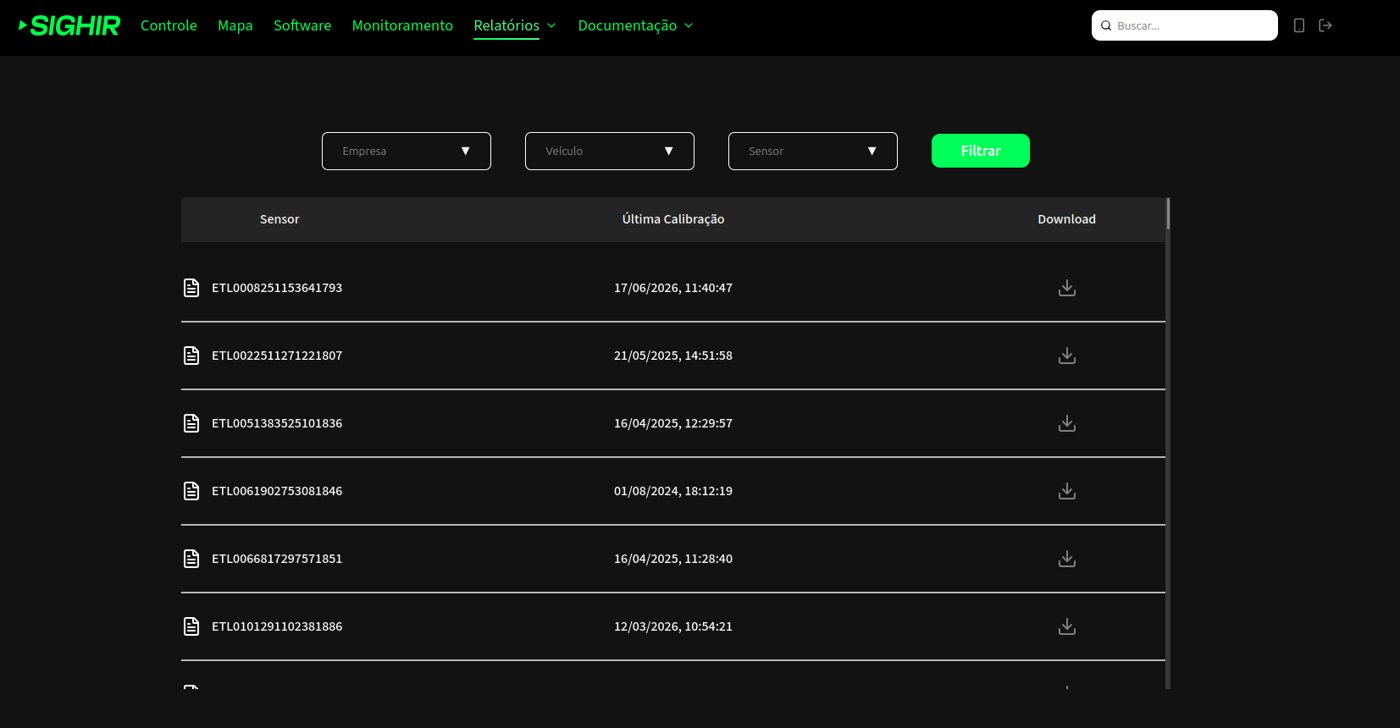
\includegraphics[width=\linewidth]{portal_calibracao.jpg}
\captionof{figure}{Portal — Relatórios de Calibração: data da última calibração e certificado em PDF por sensor.}
\end{center}
\end{multicols}

% =====================================================================
%  PÁGINA 8 — SEGURANÇA E FRAUDES
% =====================================================================
\section{Segurança e prevenção de fraudes}

O DAD01 combina barreiras físicas, lógicas e de auditoria. Qualquer tentativa de realizar o
teste fora do procedimento normal é \textbf{reconhecida pelo equipamento e gera um evento
específico}, visível ao gestor no portal.

\footnotesize
\renewcommand{\arraystretch}{1.32}
\begin{tabularx}{\linewidth}{@{}B{43mm}LP{27mm}@{}}
\headrow \thead{Tentativa ou desvio} & \thead{Como o equipamento reage} & \thead{Evidência}\\
Soprar fraco, intermitente ou não soprar & Sopro não reconhecido pela IA e coleta reiniciada; sem sopro válido em 25\,s o teste termina sem liberar o veículo & \ev{11}\\
\rowcolor{slight} Sopro simulado (bomba, compressor, ar de outra fonte) & A IA de sopro exige padrão de pressão compatível com sopro humano contínuo, com 7 confirmações consecutivas & coleta reiniciada / \ev{11}\\
Outra pessoa sopra na partida & Testes randômicos durante a viagem; vídeo do teste nas frotas com câmera integrada & \ev{12}, \ev{25}, vídeo\\
\rowcolor{slight} Recusar ou ignorar o teste randômico & Alarme visual e sonoro por até 3 minutos; em seguida, \emph{Motorista Não Autorizado} com alarme contínuo e bloqueio ao desligar & \ev{33}, \ev{35}, \ev{02}\\
Adiar repetidamente & Número máximo de adiamentos por teste; esgotado o limite, o teste é obrigatório & \ev{15}, \ev{34}\\
\rowcolor{slight} Tentar adivinhar a contrassenha & Desafio numérico diferente a cada liberação, máximo de 3 tentativas, resposta gerada apenas em conta autorizada & \ev{40} (código digitado)\\
Remover, desconectar ou trocar o sensor & Sem sensor válido o equipamento não conclui a inicialização e o veículo permanece bloqueado; a troca é identificada pelo número de série & \ev{24}, \ev{36}\\
\rowcolor{slight} Desligar ou reiniciar o equipamento & O equipamento reinicia bloqueado; reinicializações e silêncio de comunicação são registrados e auditados & \ev{08}\\
Dar partida sem fazer o teste & Partida bloqueada no circuito de ignição; com MiX 2.0, ignição ligada sem teste e sem viagem é bloqueada em 70\,s & \ev{02}\\
\rowcolor{slight} Romper a comunicação com o rastreador & Teste de comunicação no autodiagnóstico; ausência de eventos detectada pela auditoria da frota & \ev{06}\\
Alterar configurações do equipamento & Wi-Fi desabilitado em operação; acesso local apenas com o aplicativo e credenciais autorizadas; toda aplicação de parâmetros é registrada & \ev{07}\\
\end{tabularx}
\normalsize
\renewcommand{\arraystretch}{1.25}

\begin{multicols}{2}
\subsection{Barreiras físicas}
\begin{itemize}
  \item Unidade embutida e chicote \textbf{ocultos atrás do painel}, com o relé no circuito de ignição — sem ponto de desconexão ao alcance do motorista.
  \item Instalação apenas por técnicos credenciados, com relatório fotográfico arquivado no portal.
\end{itemize}

\subsection{Auditoria contínua da frota}
A SIGHIR mantém uma rotina de \textbf{auditoria automática} sobre os eventos de toda a frota,
que classifica as ocorrências em 12 categorias — entre elas \emph{álcool detectado},
\emph{tentativa de burla do bloqueio}, \emph{conduta do motorista} (adiamentos frequentes),
\emph{testes inconclusivos}, \emph{sem comunicação}, \emph{calibração vencida} e
\emph{defeito do aparelho} — e acompanha cada caso até a solução. Padrões anormais também são
destacados no painel \textbf{Últimos Eventos de Alerta}.

\columnbreak
\subsection{Evidência: trilha real de eventos}
Registro de produção de 16/09/2026 (veículo omitido), com o horário do equipamento e o de
recebimento no servidor:

\footnotesize
\begin{tabularx}{\linewidth}{@{}P{11.5mm}P{11.5mm}P{20mm}L@{}}
\headrow \thead{Equip.} & \thead{Servidor} & \thead{Evento} & \thead{Significado}\\
13:05:27 & 13:05:28 & \texttt{\$ETEV05!} & Sopro realizado\\
\rowcolor{slight} 13:05:46 & 13:05:48 & \texttt{\$ETEV300494!} & \textcolor{salert}{\textbf{Álcool: 0,494\,mg/L}}\\
13:05:51 & 13:05:53 & \texttt{\$ETEV16!} & Teste realizado\\
\rowcolor{slight} 13:05:54 & 13:05:56 & \texttt{\$ETEV02!} & \textbf{Veículo bloqueado}\\
13:17:14 & 13:17:17 & \texttt{\$ETEV05!} & Novo sopro, após a purga\\
\rowcolor{slight} 13:17:34 & 13:17:36 & \texttt{\$ETEV29!} & Leitura sem álcool\\
13:17:37 & 13:17:39 & \texttt{\$ETEV16!} & Teste realizado\\
\rowcolor{slight} 13:17:40 & 13:17:42 & \texttt{\$ETEV01!} & Veículo desbloqueado\\
13:51:53 & 13:51:55 & \texttt{\$ETEV17!} & Tempo de manobra\\
\rowcolor{slight} 13:56:55 & 13:56:57 & \texttt{\$ETEV18!} & Fim do tempo de manobra\\
13:57:01 & 13:57:04 & \texttt{\$ETEV02!} & Veículo bloqueado\\
\end{tabularx}
\normalsize
\end{multicols}

% =====================================================================
%  PÁGINA 9 — REGISTRO DE EVENTOS
% =====================================================================
\section{Registro e rastreabilidade de eventos}

\begin{multicols}{2}
\subsection{Como os eventos são registrados}
Cada ocorrência gera um \textbf{evento codificado} (\ev{nn}) que o equipamento transmite
imediatamente ao rastreador pela RS232. A telemetria entrega o evento ao servidor SIGHIR, em
nuvem, que o associa ao equipamento, ao veículo e à empresa. O equipamento também mantém um
\textbf{registro local} dos eventos mais recentes, consultável pelo aplicativo via Wi-Fi.

\subsection{Identificação do equipamento}
Cada evento armazenado traz:
\begin{itemize}
  \item \textbf{número de série do equipamento} (ID único \texttt{MIC…}) e \textbf{ID do sensor} (\texttt{ETL…}, gravado em fábrica);
  \item \textbf{placa}, empresa e telemetria do veículo;
  \item \textbf{data e hora do equipamento} e \textbf{data e hora de recebimento} no servidor;
  \item \textbf{posição GPS} informada pelo rastreador, quando disponível.
\end{itemize}

\subsection{Identificação de quem realizou a operação}
\begin{itemize}
  \item \textbf{Motorista:} identificação de condutor da telemetria, quando habilitada, e vídeo do teste nas frotas com câmera integrada.
  \item \textbf{Operações na plataforma} (bloqueio/desbloqueio remoto, parâmetros, firmware): usuários com \textbf{credenciais individuais}, registrados com usuário, data/hora e origem do acesso.
  \item \textbf{Liberação por contrassenha:} cada código digitado fica registrado; a resposta só é gerada em conta de supervisor autorizado.
  \item \textbf{Instalação e troca de sensor:} relatório com o técnico responsável e o ID do sensor.
\end{itemize}

\subsection{Armazenamento e retenção}
Os eventos são armazenados no servidor SIGHIR \textbf{sem expurgo automático}: todo o histórico
desde a implantação da plataforma atual (julho de 2025) permanece disponível para consulta. A
plataforma da telemetria mantém uma cópia independente, conforme a política do provedor.

\subsection{Integridade dos registros}
\begin{itemize}
  \item Portal e API de consulta são \textbf{somente leitura} para o cliente: não há função de edição ou exclusão de eventos.
  \item O servidor carimba o \textbf{horário de recebimento} de cada evento, independente do relógio do equipamento.
  \item A cópia mantida pela telemetria permite \textbf{confronto independente} dos registros.
  \item O acesso administrativo à base é restrito à equipe SIGHIR e registrado em trilha de auditoria.
\end{itemize}

\end{multicols}

\subsection{Eventos registrados}
\footnotesize
\renewcommand{\arraystretch}{1.13}
\begin{minipage}[t]{0.485\textwidth}
\begin{tabularx}{\linewidth}[t]{@{}P{31mm}L@{}}
\headrow \thead{Código} & \thead{Evento}\\
\grupo{Teste de alcoolemia}
\ev{05} & Sopro realizado\\
\ev{29} & Leitura sem álcool\\
\ev{30mgl} & Álcool detectado, com a concentração\\
\ev{16} · \ev{25} & Teste realizado · randômico realizado\\
\ev{11} & Sem sopro\\
\ev{15} & Teste adiado\\
\grupo{Teste randômico}
\ev{12} · \ev{34} & Randômico solicitado · adiado\\
\ev{33} & Randômico não realizado\\
\ev{35} & Motorista não autorizado\\
\grupo{Veículo e liberações}
\ev{01} · \ev{02} & Veículo desbloqueado · bloqueado\\
\ev{37} · \ev{38} & Bloqueio · desbloqueio remoto\\
\ev{04} & Veículo desligado\\
\ev{17} · \ev{18} & Início · fim do tempo de manobra\\
\ev{22} · \ev{32} & Manobrista ativado · partida no modo\\
\ev{40cod} · \ev{26} & Contrassenha digitada · aceita\\
\end{tabularx}
\end{minipage}\hfill
\begin{minipage}[t]{0.485\textwidth}
\begin{tabularx}{\linewidth}[t]{@{}P{31mm}L@{}}
\headrow \thead{Código} & \thead{Evento}\\
\grupo{Sensor}
\ev{09id} & Sensor inicializado (número de série)\\
\ev{36id} & Sensor substituído (novo número)\\
\ev{13nnnn} & Sensor próximo do vencimento\\
\ev{14nnnn} & Sensor vencido\\
\ev{20} · \ev{24} & Autodiagnóstico ok · sensor defeituoso\\
\grupo{Sistema e ambiente}
\ev{08} & Dispositivo inicializado\\
\ev{06} & Falha de comunicação com a telemetria\\
\ev{07} & Parâmetros atualizados\\
\ev{10} & Firmware atualizado\\
\ev{27} · \ev{28} & Temperatura alta · crítica\\
\ev{41} & Umidade alta\\
\end{tabularx}
\normalsize
\begin{alerta}
O conjunto de eventos visível no portal depende da integração de cada telemetria. Suntech e
Entrack repassam a totalidade dos eventos; na MiX Telematics, o repasse segue o script de
integração configurado no rastreador.
\end{alerta}
\end{minipage}
\renewcommand{\arraystretch}{1.25}

% =====================================================================
%  PÁGINA 10 — CONSULTA E RELATÓRIOS
% =====================================================================
\subsection{Consulta, extração e relatórios}

\begin{minipage}[t]{0.49\textwidth}\centering
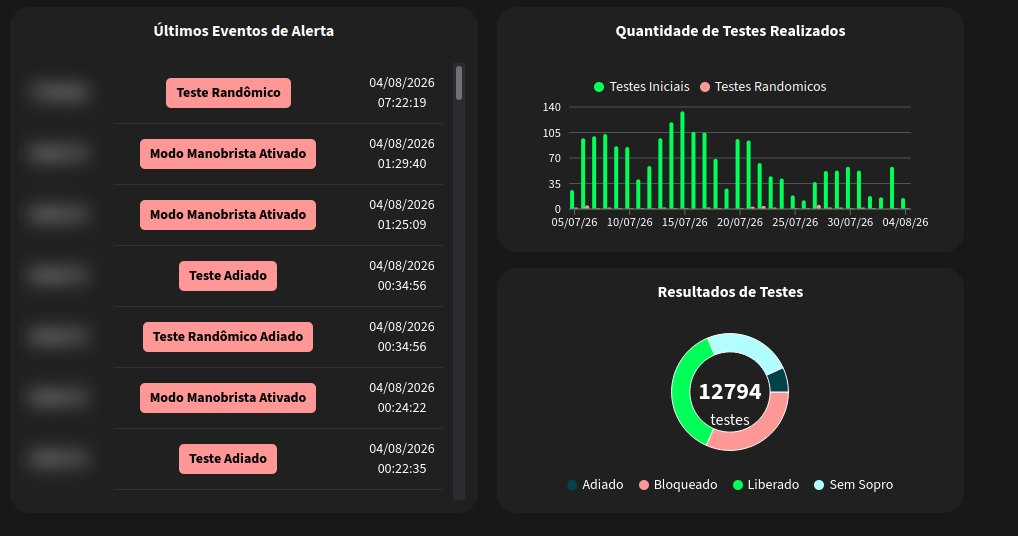
\includegraphics[width=\linewidth]{portal_controle.jpg}
\captionof{figure}{Painel de Controle: testes iniciais × randômicos, resultados e alertas (placas ocultadas).}
\end{minipage}\hfill
\begin{minipage}[t]{0.49\textwidth}\centering
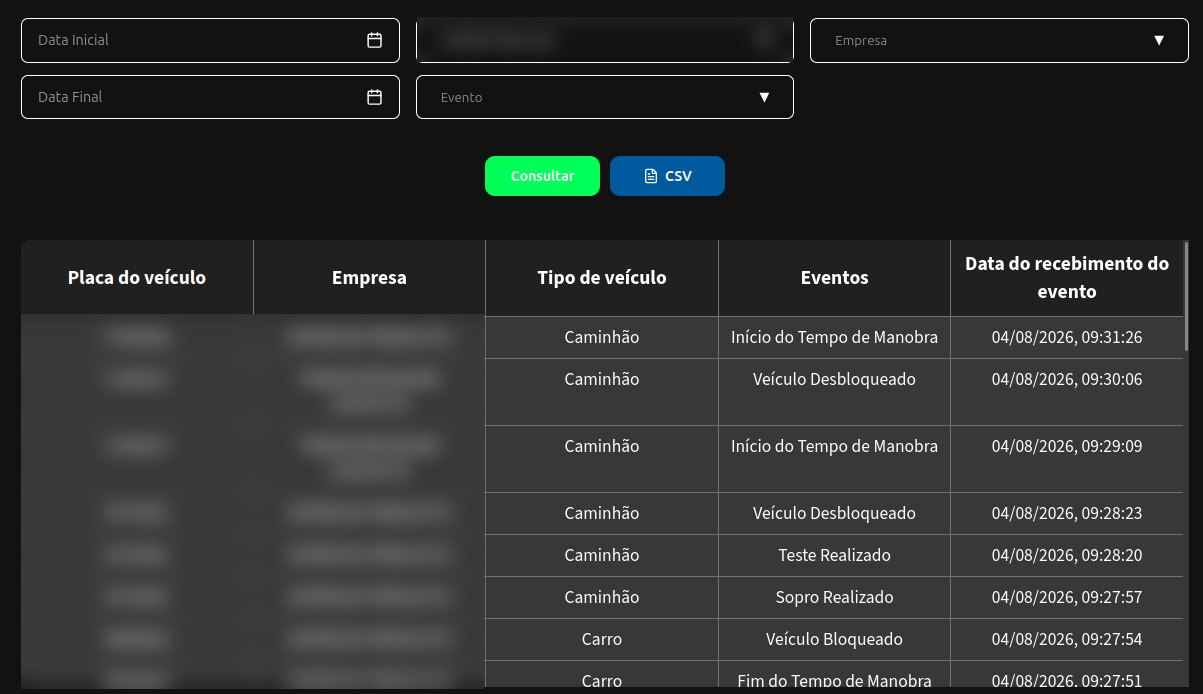
\includegraphics[width=\linewidth]{portal_monitoramento.jpg}
\captionof{figure}{Monitoramento: histórico filtrável e exportação em CSV (placas e empresas ocultadas).}
\end{minipage}

\vspace{4mm}
\small
\renewcommand{\arraystretch}{1.3}
\begin{tabularx}{\linewidth}{@{}B{40mm}L@{}}
\headrow \thead{Recurso} & \thead{O que oferece}\\
Portal — Controle & Visão da frota: última sincronização, dispositivos instalados e em estoque, \textbf{sensores vencidos}, gráfico diário de testes iniciais e randômicos, distribuição dos resultados (liberado, bloqueado, adiado, sem sopro), \textbf{últimos eventos de alerta} e exportação dos dados filtrados\\
\rowcolor{slight} Portal — Monitoramento & Histórico completo de eventos por placa, empresa, tipo de evento e período, com \textbf{exportação em CSV} para auditorias\\
Portal — Relatórios & \textbf{Certificados de calibração} em PDF por sensor e \textbf{relatórios de instalação} com fotos, checklist e técnico responsável\\
\rowcolor{slight} Portal — Mapa & Última posição de cada veículo, a partir do GPS do rastreador\\
Portal — Software & Versão de firmware vigente, notas de liberação, atualização remota e configuração de parâmetros\\
\rowcolor{slight} API REST & Integração com sistemas do cliente (autenticação por token): eventos com filtros por período, veículo, tipo de evento e telemetria; indicadores consolidados e eventos de alerta\\
Vídeo dos eventos & Nas frotas com câmera integrada, link do vídeo de cada teste, bloqueio e desbloqueio\\
\rowcolor{slight} Aplicativo SIGHIR Monitor & Leitura local do registro de eventos do equipamento e acompanhamento em tempo real dos sensores\\
\end{tabularx}
\normalsize
\renewcommand{\arraystretch}{1.25}

\vspace{4mm}
\begin{minipage}[c]{0.38\textwidth}
\setlength{\parskip}{5pt}
\subsection*{Aplicativo SIGHIR Monitor}
Ferramenta de campo para instaladores, técnicos e supervisores. Conecta-se ao equipamento pela
rede Wi-Fi própria dele e exige login com as mesmas credenciais do portal. Os recursos
dependem do perfil do usuário:
\begin{itemize}
  \item \textbf{Instalador:} instalação guiada, com checklist, fotos, parâmetros da empresa, placa e ordem de serviço assinada.
  \item \textbf{Técnico:} parâmetros, logs, monitoramento dos sensores, troca de sensor e atualização de firmware.
  \item \textbf{Supervisor autorizado:} geração da contrassenha após um positivo.
\end{itemize}
\end{minipage}\hfill
\begin{minipage}[c]{0.58\textwidth}\centering
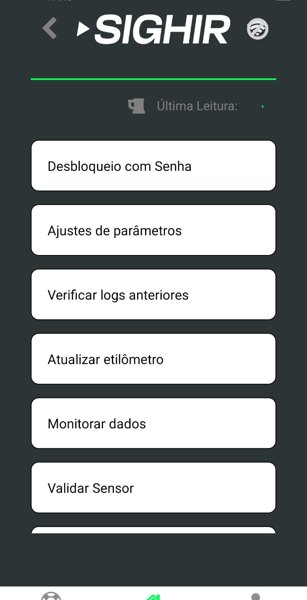
\includegraphics[height=64mm]{app_config.jpg}\hfill
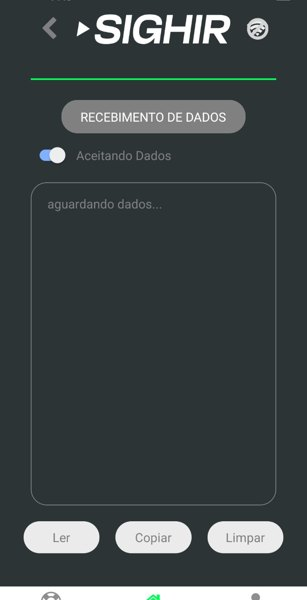
\includegraphics[height=64mm]{app_logs.jpg}\hfill
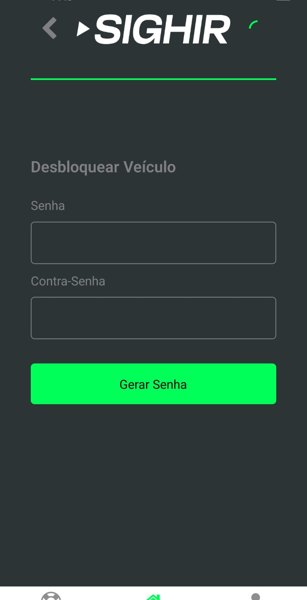
\includegraphics[height=64mm]{app_desbloqueio.jpg}
\captionof{figure}{Aplicativo: configurações, leitura de logs e geração de contrassenha.}
\end{minipage}

\begin{nota}
\textbf{Integração com videomonitoramento embarcado.} Nas frotas com câmera de parceiro homologado,
cada evento relevante (sopro, bloqueio, desbloqueio) é publicado automaticamente como ocorrência
no sistema de vídeo, e o portal SIGHIR recupera o link da gravação do instante exato do evento. A
integração é assíncrona: uma indisponibilidade do sistema de câmeras nunca impede a gravação do
evento no servidor SIGHIR.
\end{nota}

% =====================================================================
%  PÁGINA 11 — CONFIGURAÇÃO E FIRMWARE
% =====================================================================
\section{Configuração, firmware e controle de alterações}\label{sec:firmware}

\footnotesize
\begin{tabularx}{\linewidth}{@{}B{34mm}P{38mm}L@{}}
\headrow \thead{Ação} & \thead{Quem pode realizar} & \thead{Como é feita e como fica registrada}\\
Critério de detecção e modelos de IA & Somente a engenharia SIGHIR & Nova versão de firmware; não é parâmetro configurável\\
\rowcolor{slight} Atualização de firmware & Somente a SIGHIR & Portal\seta Software, por número de série; registro \ev{10} e versão reportada ao servidor\\
Parâmetros de operação & SIGHIR ou administrador autorizado & Portal\seta Configurar Parâmetros, ou aplicativo durante a instalação; registro \ev{07}\\
\rowcolor{slight} Bloqueio / desbloqueio remoto & Gestor autorizado da frota & Portal\seta Alterar Estado de Bloqueio; \ev{37}/\ev{38} com usuário, data/hora e origem\\
Liberação após positivo & Supervisor com conta autorizada & Contrassenha gerada no aplicativo; \ev{40} (cada tentativa) e \ev{26}\\
\rowcolor{slight} Troca de sensor & Técnico credenciado & Aplicativo\seta Validar Sensor; \ev{36} com o novo número de série\\
Consulta de eventos e relatórios & Usuários da empresa & Portal e API, somente leitura, segregados por empresa\\
\end{tabularx}
\normalsize

\begin{multicols}{2}
\subsection{Parâmetros configuráveis}
\footnotesize
\begin{tabularx}{\linewidth}{@{}B{27mm}LP{13mm}@{}}
\headrow \thead{Parâmetro} & \thead{Descrição} & \thead{Padrão}\\
Tempo de manobra & Religar sem novo teste após desligar & 5 min\\
\rowcolor{slight} Máximo de adiamentos & Adiamentos permitidos por teste & 3\\
Tempo de adiamento & Prazo liberado ao adiar & 5 min\\
\rowcolor{slight} Modo randômico & Testes durante a viagem & ativo\\
Testes por viagem & Quantidade de testes randômicos & 1\\
\rowcolor{slight} Adiamento do randômico & Prazo ao adiar um randômico & 5 min\\
Tempo de câmera & Espera para a câmera registrar o teste & 5 s\\
\rowcolor{slight} Modo manobrista & Uso administrativo em pátio & inativo\\
Tipo de veículo & Caminhão ou veículo leve & caminhão\\
\rowcolor{slight} Telemetria & MiX, MiX 2.0, Suntech ou Entrack & conforme a frota\\
\end{tabularx}
\normalsize

{\small Os valores padrão podem ser ajustados por empresa, conforme a política de segurança
da transportadora. O critério de detecção \textbf{não} faz parte dos parâmetros.}

\subsection{Registro das alterações}
\begin{itemize}
  \item Os eventos \textbf{Parâmetros Atualizados} (\ev{07}) e \textbf{Firmware Atualizado} (\ev{10}) registram a data e a hora de cada aplicação no equipamento.
  \item Ao se conectar, o equipamento informa ao servidor a \textbf{versão de firmware} em execução; o catálogo de versões guarda número, data de liberação e notas de cada release.
  \item Operações na plataforma ficam associadas ao \textbf{usuário autenticado}, com data/hora e origem do acesso.
\end{itemize}

\columnbreak
\subsection{Proteção contra alterações não autorizadas}
\begin{itemize}
  \item \textbf{Sem acesso remoto direto ao equipamento:} em operação o Wi-Fi permanece desligado e a RS232 fica oculta, ligada apenas ao rastreador.
  \item \textbf{Configuração local} somente com presença física, rede própria do equipamento protegida por senha e aplicativo com login de perfil autorizado.
  \item \textbf{Configuração remota} somente a partir do servidor SIGHIR: o equipamento busca parâmetros apenas no servidor oficial, por conexão HTTPS, identificado pelo seu número de série.
  \item \textbf{Firmware} publicado exclusivamente pela SIGHIR: o equipamento só baixa uma versão quando a atualização é autorizada para aquele número de série; a imagem é gravada em partição separada e validada antes de ser ativada, preservando a versão anterior em caso de falha.
  \item \textbf{Portal} com login individual, sessão com expiração automática e segregação por empresa.
\end{itemize}

\subsection{Ciclo controlado de uma atualização}
\begin{center}
\begin{tikzpicture}[
  etapa/.style={draw=tdline,line width=0.55pt,fill=white,
    text width=66mm,align=left,font=\footnotesize,inner sep=4pt,minimum height=9mm},
  num/.style={circle,draw=tdline,line width=0.55pt,fill=white,text=tdline,font=\scriptsize\bfseries,inner sep=1pt,minimum size=5mm},
  seta/.style={-{Stealth[length=1.8mm,width=1.1mm]},line width=0.55pt,tdline}]
  \node[etapa] (a) {\textbf{Desenvolvimento e testes} — a engenharia SIGHIR valida a nova versão};
  \node[etapa,below=3.5mm of a] (b) {\textbf{Publicação} — catálogo com número de versão, data e notas};
  \node[etapa,below=3.5mm of b] (c) {\textbf{Autorização} — a SIGHIR seleciona os equipamentos no portal};
  \node[etapa,below=3.5mm of c] (d) {\textbf{Instalação} — download do servidor oficial, validação da imagem e ativação};
  \node[etapa,below=3.5mm of d] (e) {\textbf{Registro} — \texttt{\$ETEV10!} e versão em execução reportada ao servidor};
  \foreach \n/\k in {a/1,b/2,c/3,d/4,e/5} \node[num] at ([xshift=-4mm]\n.west) {\k};
  \draw[seta] (a) -- (b); \draw[seta] (b) -- (c); \draw[seta] (c) -- (d); \draw[seta] (d) -- (e);
\end{tikzpicture}
\end{center}


\end{multicols}



% =====================================================================
%  PÁGINA 12 — INSTALAÇÃO, GARANTIA, DOCUMENTAÇÃO
% =====================================================================
\section{Instalação, uso seguro e garantia de funcionamento}

\begin{multicols}{2}
\subsection{Instalação}
\begin{enumerate}
  \item Realizada por \textbf{técnico credenciado}, com a chave geral desligada e o sistema antifurto do veículo desativado.
  \item \textbf{Unidade embutida} fixada em superfície plana e oculta atrás do painel, com os cabos protegidos.
  \item \textbf{Alimentação} direta da bateria com fusível dedicado; RS232 conectada à telemetria.
  \item \textbf{Relé de bloqueio no fio de pós-chave (ignição)}, pinos 30 e 87a. Nunca bloquear pela bomba de combustível ou por circuitos que possam desligar o motor em movimento.
  \item \textbf{Unidade exposta} firme, ao alcance do motorista e longe de sol direto.
  \item Configuração pelo aplicativo SIGHIR Monitor: telemetria, parâmetros da empresa e placa.
  \item \textbf{Validação obrigatória:} teste negativo libera a partida; ao desligar inicia o tempo de manobra; esgotado o prazo, o veículo bloqueia e não dá partida; o adiamento devolve o teste no prazo.
  \item Relatório de instalação com fotos e checklist enviado ao portal.
\end{enumerate}

\columnbreak
\subsection{Orientações ao motorista}
\begin{itemize}
  \item Soprar de forma firme e contínua até o fim do bipe.
  \item Não usar enxaguante bucal, sprays, balas ou gomas fortes antes do teste; se usou, aguardar alguns minutos e beber água.
  \item Evitar produtos com álcool na cabine (limpeza, perfume, álcool em gel) e mantê-la ventilada.
  \item Fazer o teste randômico assim que for seguro; parar o veículo se o alarme for acionado.
\end{itemize}

\subsection{Garantia de funcionamento}
\begin{itemize}
  \item \textbf{Teste funcional de 100\,\% dos equipamentos} em bancada antes da expedição: alimentação, display, sensores, relé e comunicação serial.
  \item \textbf{Autodiagnóstico} no menu: teste de sopro, de componentes, de relé e de comunicação com a telemetria.
  \item \textbf{Supervisão contínua} de temperatura, umidade, integridade do sensor e estabilidade da alimentação, com alertas registrados.
  \item \textbf{Monitoramento da frota} pela SIGHIR: equipamentos sem comunicação, com calibração vencida ou com defeito são identificados e tratados pelo suporte técnico.
\end{itemize}
\end{multicols}

\vfill
\begin{tcolorbox}[enhanced,colback=slight,colframe=slight,arc=1.5mm,left=5mm,right=5mm,top=4mm,bottom=4mm]
\begin{minipage}[c]{0.18\textwidth}
\includegraphics[width=\linewidth]{logo.png}\end{minipage}\hfill
\begin{minipage}[c]{0.76\textwidth}\small
\textbf{SIGHIR} — Duque de Caxias/RJ \,·\, \textbf{sighir.com} \,·\, \textbf{contato@sighir.com.br}\\[1mm]
{\scriptsize\color{sgray}\textbf{Documentação complementar} (portal, menu Documentação): PPTC 0001-01 protocolo
de comunicação · PPTC 0001-02 calibração e incerteza · INST 0001-02 instalação · MUWP 0001-01 portal web ·
MUAM 0001-01 aplicativo · manual do motorista. Telas reproduzidas conforme o firmware \fw. Informações
sujeitas a alteração sem aviso prévio.}
\end{minipage}
\end{tcolorbox}

\end{document}
